%!TEX root = ../thesis.tex
\newchap{The CMS experiment at LHC}\label{sec:CMS}
\minitoc

CERN is the largest international particle physics research center in the world. It is located across the Franco-Swiss border in Meyrin, near Geneva, and was founded in 1954, after the end of the World War II, by twelve European countries.\\
Today, more than 100 countries, 500 institutes, and 13000 users collaborate to the CERN activities.

\section{The Large Hadron Collider}
The CERN's major facility is the Large Hadron Collider (LHC), a proton-proton (pp) and lead ion (Pb-Pb) collider that, with its lengths of 26.7 km and its energy in the center of mass of $\sqrt{s}=14\TeV$, is the largest and the most powerful particle accelerator ever built in the world.\\
As shown in \Fig{fig:cern}, the LHC is just the last stage of a chain of accelerators. The protons obtained ionizing hydrogen are grouped in bunches through a quadrupole magnet and then are sent to a chain of accelerators that increase progressively the energy of the protons.
Before entering the LHC, the proton beam is split into two beam lines that travel in opposite direction and then are accelerated by radiofrequency (RF) cavities that are tuned to oscillate at 400MHz. In addition to RF cavities, quadrupoles are used to keep the beam focused and dipoles to bend the beam \cite{Bruning2004LHCReport}.\\
Once the beam is stabilized, the proton bunches collide in four different points where the experiments ATLAS, CMS, LHCb and ALICE are located.\\
ATLAS (A Toroidal LHC ApparatuS) and CMS (Compact Muon Solenoid) are general purpose detectors and are the ones that in the 2012 discovered the Higgs boson  \cite{Chatrchyan2012ObservationLHC,Aad2012ObservationLHC}, LHCb (LHC beauty) is a forward detector designed to study the physics of the B mesons and the matter-antimatter asymmetry and ALICE (A Large Ion Collider Experiment) is a detector devoted to the study of quark-gluon plasma and extreme phases of QCD matter through the analysis of lead ion collisions.
\begin{figure}[h!]
    \centering
    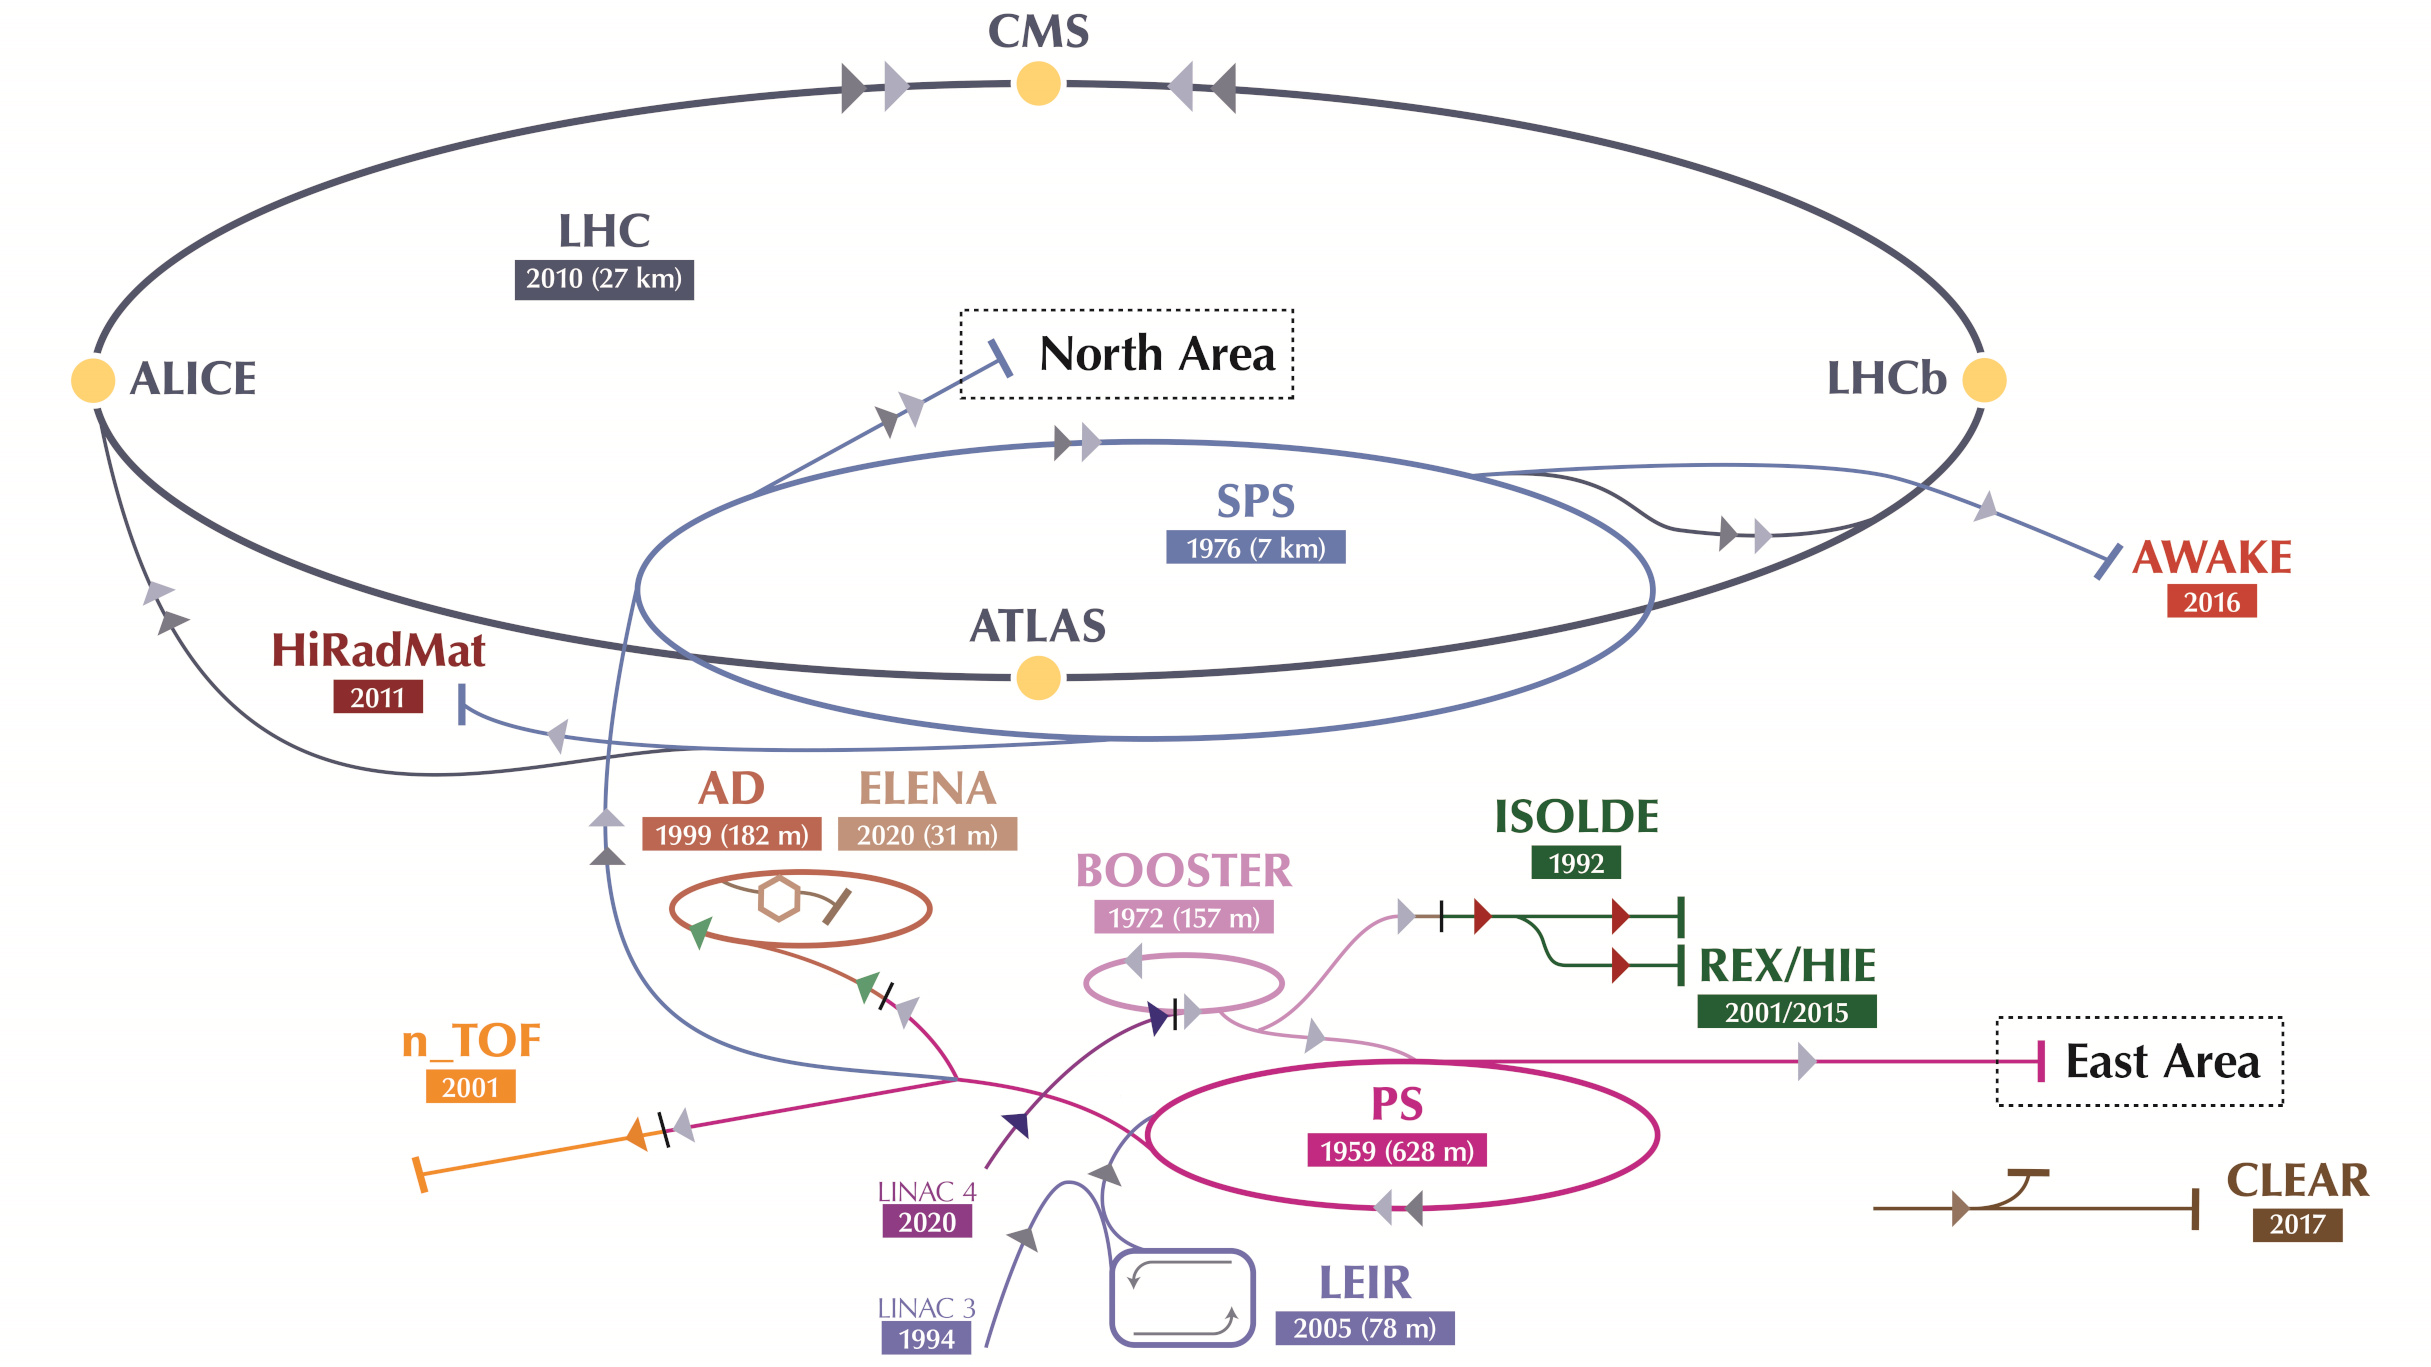
\includegraphics[width=\textwidth]{fig//chap03-cms/cern.jpg}
    \caption{CERN's accelerator complex. The accelerating chain is: LINAC2 (50 \MeV) $\to$ Booster (1.4\GeV) $\to$ Proton Synchrotron (PS) (26\GeV) $\to$ Super Proton Synchrotron (450\GeV) $\to$ LHC (13/14 \TeV). The intermediate accelerators also provide a proton beam to other smaller experiments and facilities. \cite{Panoramas}}
    \label{fig:cern}
\end{figure}

\paragraph*{Luminosity}
The \emph{instantaneous luminosity} is defined as the ratio between the event rate produced for a given process and its cross-section
\begin{equation}
    \mathcal{L} = \frac{\partial N}{\partial t} \frac{1}{\sigma} 
\end{equation}
and can be expressed also as a function of the beam parameters
\begin{equation}
    \mathcal{L}=\frac{N_{p}^{2}f\gamma_{r}}{4\pi\epsilon_{n}\beta\sp{\ast}}F\ 
\end{equation}
where $N_p$ is the number of protons per bunch, $f$ the bunch frequency, $\gamma_r$ the relativistic factor, and $\epsilon_n, \beta^*, F$ are geometrical factors that take into account the shape of the beam and the crossing angle between the two beams in the interaction point.\\
These parameters depend on the so-called “filling scheme”, the chosen pattern of filled and empty bunch crossings used in a single fill.
A typical filling scheme is composed of long strings of consecutive bunches called a “train”, with the individual trains separated by gaps of varying lengths. Filling schemes also include some number of non-colliding bunch crossings that can be used to study effects from beam-induced background \cite{CMSCollaboration2021PrecisionCMS}.\\
The LHC was designed to achieve an instantaneous luminosity of $\mathcal{L}=10^{34} cm^{-2}s^{-1}$ but, in 2018, the LHC was able to reach a peak luminosity of $\mathcal{L}=2.1 \cdot 10^{34} cm^{-2}s^{-1}$ doubling the nominal design value. Increasing the luminosity is essential to observe rare events and to decrease the statistical uncertainties of every analysis, but it has a drawback: the number of simultaneous pp interactions, called pileup (PU), increase with the instantaneous luminosity, making the event reconstruction more difficult. PU effects can be mitigated thanks to high granularity detectors and advanced reconstruction algorithms.\\
The amount of recorded data is quantified by the \emph{integrated luminosity}, the time integral of the instantaneous luminosity $\mathcal{L}_I=\int dt \mathcal{L}(t)$.


\begin{figure}[h!]
    \centering
    \begin{minipage}{0.52\linewidth}
        
        \centering
        \includegraphics[width=\linewidth]{fig//chap03-cms/lumi.png}
        (a)
    \end{minipage}
    \begin{minipage}{0.47\linewidth}
        \vspace{0.6cm}
        \centering
        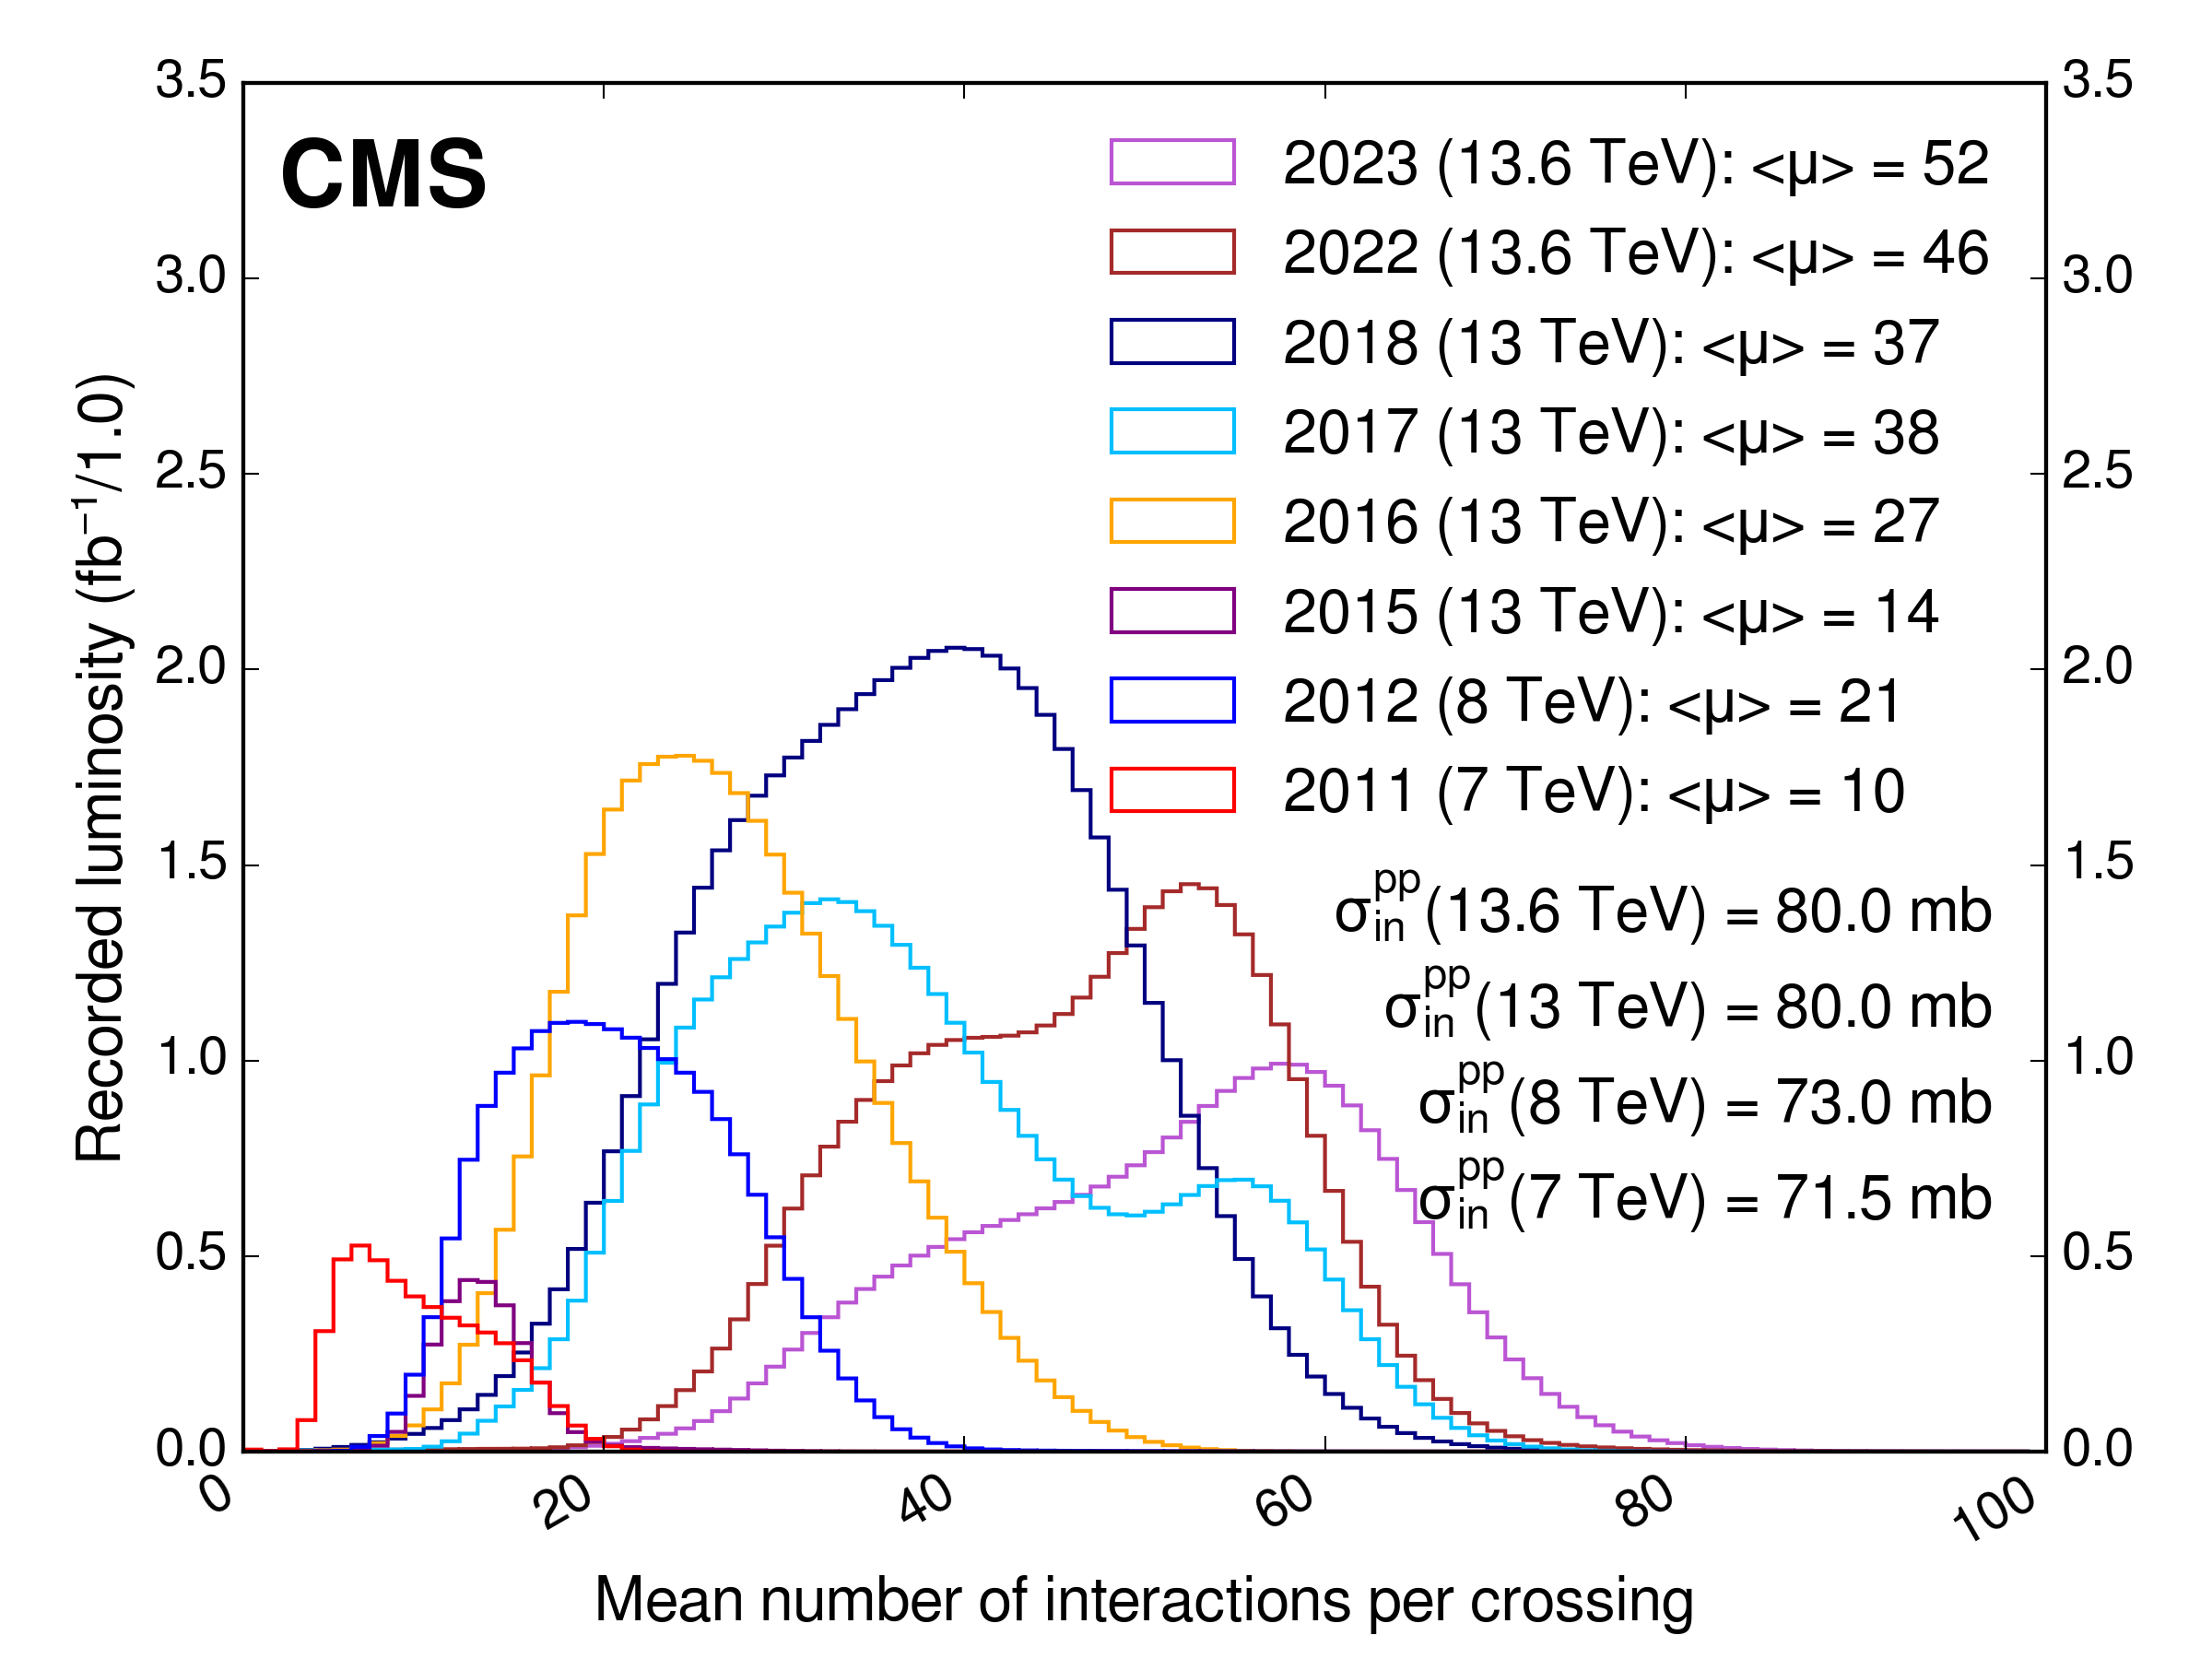
\includegraphics[width=\linewidth]{fig//chap03-cms/pileup.png}
        (b)
    \end{minipage}
    \caption{(a) cumulative integrated luminosity delivered and recorded by the CMS experiment; (b) PU distribution across different years at the CMS experiment \cite{LumiPublicResultsTWiki}}
    \label{fig:lumi_pu}
\end{figure}
\paragraph*{Physics runs}
The LHC program covers a period of $\sim$ 30 years, divided into two phases. 
The \emph{Phase I} includes the Run I (2011-2012), the Run II (2015-2018) and the Run III (2022-2025).
During the Phase I the center of mass energy was increased from $7 \TeV$ to $13.6 \TeV$ and the instantaneous luminosity reached a peak of $\mathcal{L}= 2.1 \cdot 10^{34}cm^{-2} s^{-1}$. \\
At the end of 2025, the LHC will enter the \emph{High Luminosity} LHC (HL-LHC) phase, a new phase of upgrades that will take the center of mass energy to 14 \TeV and to an instantaneous luminosity of $\mathcal{L}=5 \cdot 10^{34}cm^{-2} s^{-1}$, providing an integrated luminosity in all the Phase II (2029-2040) of $\mathcal{L}_I=3000 fb^{-1}$, ten times more than in Phase I.\\
During the long shutdown 3 (LS3: 2025-2029) the detectors will be upgraded, along the LHC, to be able to work in such a challenging environment that causes more radiation damage, specially in the forward subdetectors, and with a significant PU increase to <PU>$\sim 200$. 

\begin{figure}[h!]
    \centering
    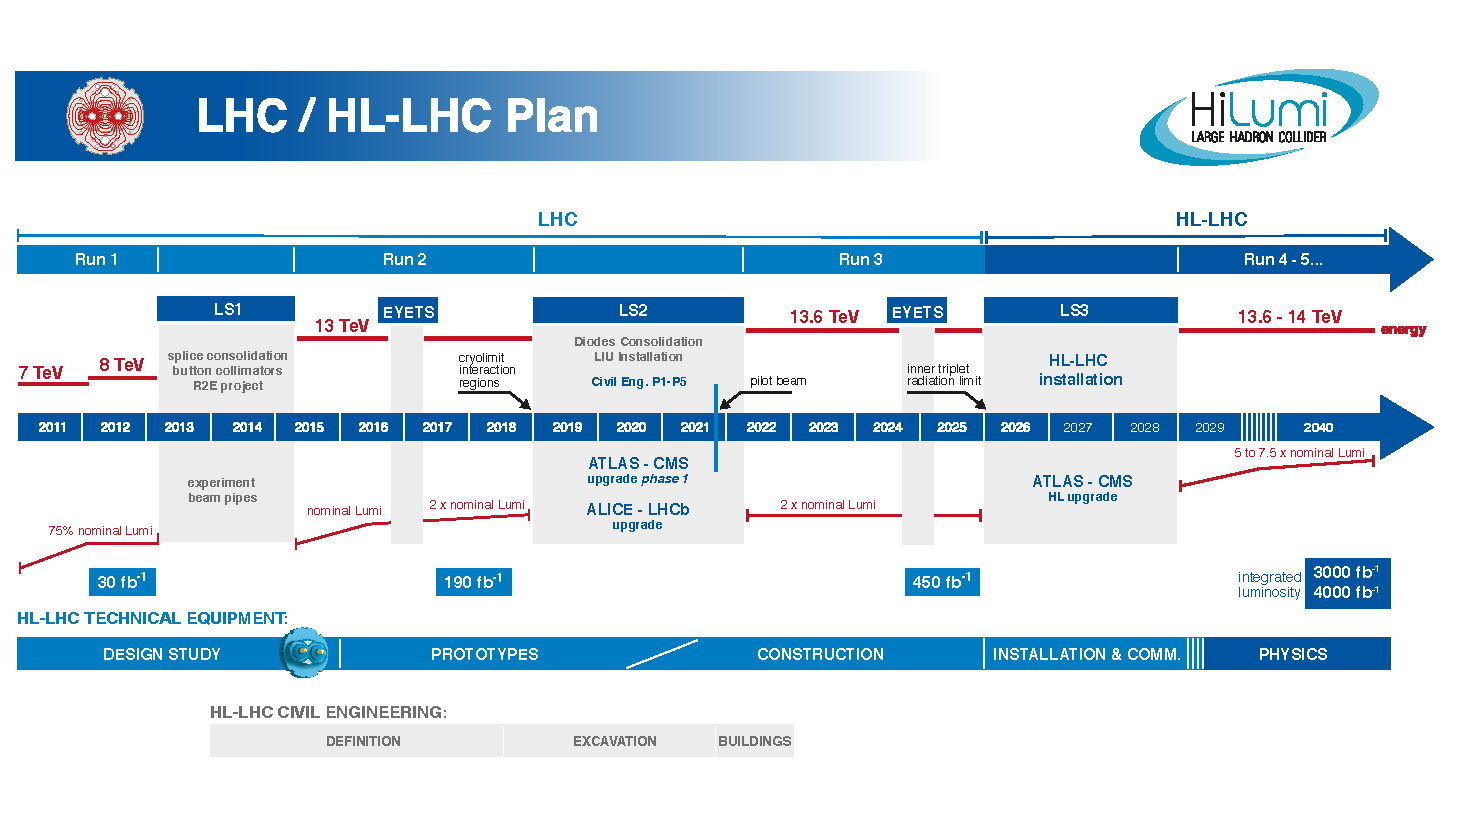
\includegraphics[width=1\linewidth]{fig//chap03-cms/LHC_schedule.pdf}
    \caption{Schedule of the LHC operations \cite{LS3Project}}
    \label{fig:lhc_schedule}
\end{figure}
\\




\section{The Compact Muon Solenoid experiment}
\subsection{Tracker}
\subsection{Electromagnetic calorimeter}
\subsection{Hadronic calorimeter}
\subsection{Muon system}
\subsection{Trigger and data acquisition}
